Coordinated Linear Meld (CLM) is a forward-chaining linear logic programming
language based on LM~\cite{cruz-iclp14}.
Programs consist of a set of \emph{rules} and a \emph{database of facts}.
Rules have the form \mytt{a(X), b(Y) -o c(X, Y)} and can be read as follows: if fact \mytt{a(X)}
and fact \mytt{b(Y)} exist in the database then \mytt{c(X, Y)} is added to
the database. The expression \mytt{a(X), b(Y)} is called the \emph{body} of
the rule and \mytt{c(X, Y)} is the \emph{head} of the rule.
A fact is a predicate, e.g., \mytt{a}, \mytt{b} or \mytt{c}, and its
associated tuple of values, e.g., the concrete values of \mytt{X} and
\mytt{Y}. Since CLM uses linear logic as its foundation, we distinguish between
\emph{linear} and \emph{persistent facts}. Linear facts are deleted during the
process of deriving a rule, while persistent facts are not.
Program execution starts by adding the \emph{axioms} (the initial facts)
to the database. Next, rules are recursively applied and the
database is updated by adding new facts or deleting facts used during rule derivation.
When no more rules are applicable, the program terminates.

CLM has been designed for writing programs that operate on graphs. To achieve
concurrency, CLM partitions the database by using the first argument of each fact. The first argument has
type \emph{node} and represents a node in the graph. For example,
the fact \mytt{f(@1, 2)} is stored in node \mytt{@1}, while
fact \mytt{p(@2)} is stored in node \mytt{@2}. CLM restricts the body of
every rule to facts with the same node so that nodes can derive rules
independently. The head of the rule may refer
to any node as long as that node is referred to somewhere in the body. This allows
\scare{communication} between nodes during rule derivation, since a node may
\scare{send} a fact to another node.  Rule restrictions in turn make CLM
implicitly parallel because nodes are able to compute independently. This makes
CLM non-deterministic since nodes can be picked to run in any order, affecting
which rules are applied and which facts are deleted or derived.

\paragraph{SSSP Example}\label{sect:ssspex}
To make these ideas concrete, Fig.~\ref{code:shortest_path_program} presents
a simple program: the single source shortest path program~(SSSP). Later in the paper, we
add coordination facts to improve the execution of this program.

The SSSP program starts (lines 1-3) with the declaration of the predicates.
Predicates specify the facts used in the program. The first predicate,
\mytt{edge}, is a persistent predicate that describes the
relationship between the nodes of the graph, where the third argument
represents the weight of the edge (the \mytt{route} modifier
informs the compiler that the \mytt{edge} predicate
determines the structure of the graph).  The predicates
\mytt{shortest} and \mytt{relax} are specified as linear facts
and thus are deleted when deriving new facts.  The algorithm computes
the shortest distance from node \mytt{@1} to all other nodes in the
graph. Every node has a \mytt{shortest} fact that is improved with
new \mytt{relax} facts.  Lines 5-9 declare the axioms of the
program: \mytt{edge} facts describe the graph; \mytt{shortest(A,
+00, [])} is the initial shortest distance (infinity) for all
nodes; and \mytt{relax(@1, 0, [@1])} starts the algorithm by
setting the distance from \mytt{@1} to \mytt{@1} to be 0.

\begin{topfig}
\scriptsize\begin{Verbatim}[numbers=left]
type route edge(node, node, int).
type linear shortest(node, int, list int).
type linear relax(node, int, list int).

!edge(@1, @2, 3). !edge(@1, @3, 1).
!edge(@3, @2, 1). !edge(@3, @4, 5).
!edge(@2, @4, 1).
shortest(A, +00, []).
relax(@1, 0, [@1]).

shortest(A, D1, P1), D1 > D2, relax(A, D2, P2)
   -o shortest(A, D2, P2),
      {B, W | !edge(A, B, W) |
         relax(B, D2 + W, P2 ++ [B])}.

shortest(A, D1, P1), D1 <= D2, relax(A, D2, P2)
   -o shortest(A, D1, P1).
\end{Verbatim}
  \scap{code:shortest_path_program}{Single Source Shortest Path program code.}
\end{topfig}

\begin{dblfig}
\vspace*{-2ex}
\begin{center}
  \subfloat[]{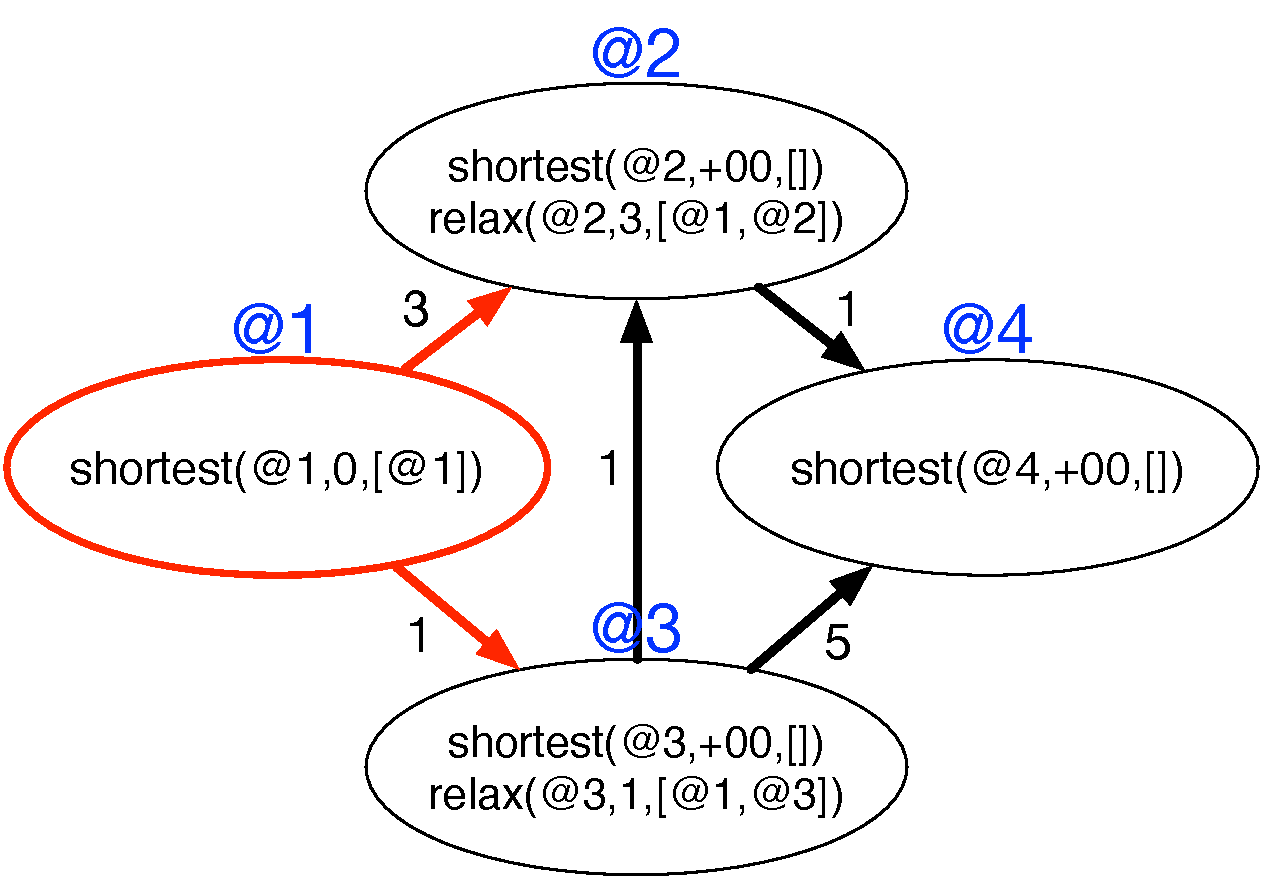
\includegraphics[width=0.3\textwidth]{figures/shortest2}}
  \hspace{0.4cm}
  \subfloat[]{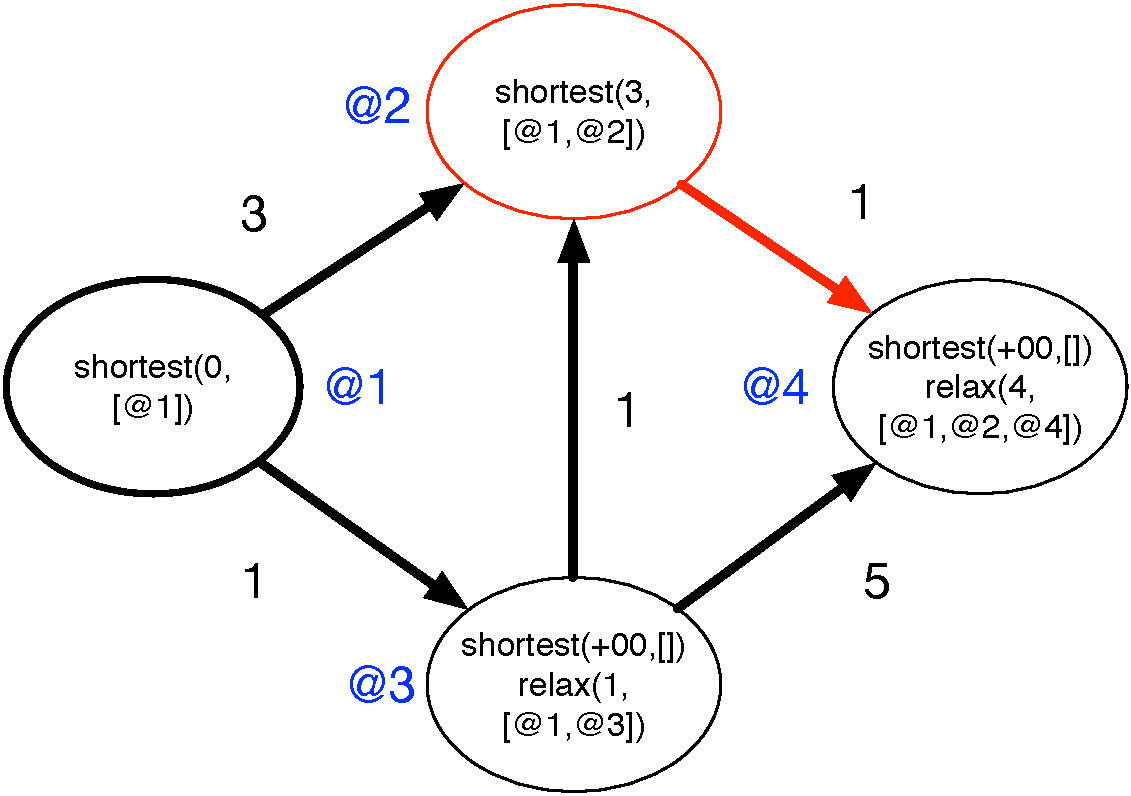
\includegraphics[width=0.3\textwidth]{figures/shortest3}}
  \hspace{0.4cm}
  \subfloat[]{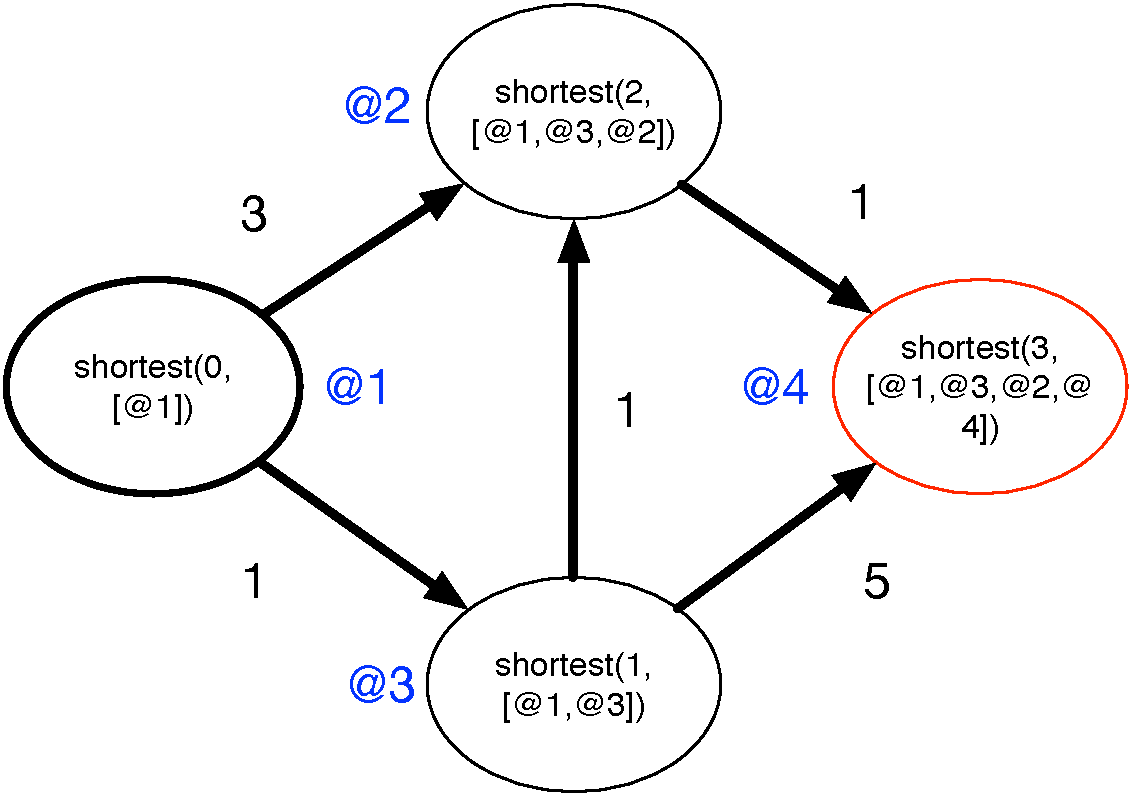
\includegraphics[width=0.3\textwidth]{figures/shortest8}}
\end{center}
\scap{fig:shortest_path_program}{Graphical representation of the SSSP program. (a) represents the
   program after propagating initial distance at node \mytt{@1}, followed by
   (b) where the first rule is applied in node \mytt{@2}. (c)
   represents the state of the final program, where all the shortest paths
   have been computed.}
\vspace*{-1ex}
\end{dblfig}

The first rule of the program (lines 11-14) reads as following: if the current
\mytt{shortest} path \mytt{P1} with distance \mytt{D1} is larger
than a new path \mytt{relax} with distance \mytt{D2}, then replace the
current shortest path with \mytt{D2}, delete the new \mytt{relax} path and
propagate new paths to the neighbors (lines 13-14) using a \emph{comprehension}.
The comprehension iterates over the edges of node \mytt{A} and derives a new
\mytt{relax} fact for each node \mytt{B} with the distance \mytt{D2 + W},
where \mytt{W} is the weight of the edge. For
example, in Fig.~\ref{fig:shortest_path_program}~(a) we apply rule 1 in node
\mytt{@1} where two new \mytt{relax} facts are derived at node \mytt{@2}
and \mytt{@3}. Fig.~\ref{fig:shortest_path_program}~(b) is the result after
applying the same rule but at node \mytt{2}.

The second rule of the program (lines 16-17) is read as following: if the
current shortest path \mytt{D1} is shorter than the new path \mytt{D2} then
delete the new \mytt{relax} fact and keep the current shortest path.

There are many opportunities for concurrency in the SSSP program. For instance,
after applying rule 1 in Fig.~\ref{fig:shortest_path_program}~(a), it is
possible to either apply rules in either node \mytt{@2} or node
\mytt{@3}. This decision depends largely on implementation factors such
as node partitioning and number of threads in the system.  Still, it is
easy to prove that no matter the scheduling used, the final result, as
presented in Fig.~\ref{fig:shortest_path_program}~(c), is achieved.

%On the other hand, CLM has no natural matching of data and computation to workers (processes, threads),
%since nodes are a program abstraction and part of the program's logic.
%We view the set of nodes as a graph data structure where workers will perform work.
%A worker is able to process any node, although a node cannot be computed by more than one worker
%at the same time. This disallows the manipulation of a node by multiple workers.
